\documentclass[serif, pdf]{beamer}

%   Theme
\usetheme{Warsaw}

%   Packages
\usepackage{xcolor}
\usepackage{tikz}
\usepackage{multimedia}
\usepackage{lmodern}
\usepackage{scrextend}
\usepackage{subcaption}
%\usepackage{media9}
%\usepackage{movie15}

%   To keep the spacing of text in tables
\usepackage{makecell}
%   Parameter for the spacing
\setcellgapes{4pt}

\usepackage{caption}
%   Redefines the caption setup of the Figures environment in the beamer class
\captionsetup[figure]{labelformat=empty}
\setbeamerfont{caption}{size=\scriptsize}

%   Colour theme
\usecolortheme{beaver}

%   Metadata
\title[SAIMechE 2019]{Virtual Evolution of 2D Soft Robots}
\date{22 November 2019}
\author[Naud\'e Conradie]{Naud\'e Conradie\\{\small Supervisor: Dr MP Venter}}
\institute[]{Department of Mechanical and Mechatronic Engineering, Stellenbosch University}

%   Colour definitions
\definecolor{colour1}{RGB}{96, 34, 59}
\definecolor{colour2}{RGB}{140, 151, 154}
\setbeamercolor{structure}{fg=colour1,bg=colour2}
\setbeamercolor{title}{fg=white,bg=colour2}
\setbeamercolor{author in head/foot}{fg=colour1}

%   Beamer template settings
\setbeamertemplate{itemize item}{\color{black}$\bullet$}
\setbeamertemplate{itemize subitem}{\color{black}$-$}
\setbeamertemplate{caption}{\raggedright\insertcaption\par}

%   Footer settings
\expandafter\def\expandafter\insertshorttitle\expandafter{%
  \insertshorttitle\hfill%
  \hspace{30mm}\insertframenumber\,/\,\inserttotalframenumber}

\beamertemplatenavigationsymbolsempty

\begin{document}

%   Title Slide-------------------------------------------------%

\begin{frame}
  \begin{center}
    \vspace{0.1cm}
    \includegraphics[scale=0.25]{USlogo.pdf}
  \end{center}
  \titlepage
\end{frame}

%   Overview----------------------------------------------------%

\changefontsizes{13pt}
\begin{frame}
    \frametitle{Overview}
    \begin{itemize}
        \item<1-> Project scope
        \item<2-> Background
        \item<3-> Methodology
        \item<4-> Results and Conclusions
    \end{itemize}
\end{frame}

%   Project Scope-----------------------------------------%

\begin{frame}
    \frametitle{Project Scope}
    \begin{itemize}
        \item<1-> Automate design of shape-changing soft robots
        \changefontsizes{11pt}
        \begin{itemize}
            \item<2-> Change internal pressure
        \end{itemize}
        \item<3-> Non-linear FEM
        \changefontsizes{11pt}
        \begin{itemize}
            \item<4-> Restricted to two dimensions
            \item<5-> Modelled with real material properties
        \end{itemize}
    \end{itemize}
\end{frame}

%   Project Scope-----------------------------------------%

\begin{frame}
    \frametitle{Project Scope (cont.)}
    \begin{itemize}
        \item<1-> Computationally efficient
        \changefontsizes{11pt}
        \begin{itemize}
            \item<2-> Use recursive grammatical encodings
            \item<3-> L-systems for cellular level
            \item<4-> CPPNs for organism level
        \end{itemize}
        \item<5-> Evolve a population to obtain best model
    \end{itemize}
\end{frame}

%   Background----------------------------------------------------%

\begin{frame}
    \frametitle{Background}
    \begin{itemize}
        \item<1-> Soft robotics
        \changefontsizes{11pt}
        \begin{itemize}
            \item<2-> Modelling and evolving soft bodies is computationally expensive
        \end{itemize}
    \end{itemize}
    \begin{figure}[ht!]
        \captionsetup{skip=0.333\baselineskip}
        \centering
        \begin{subfigure}{.23\textwidth}
            %\centering
            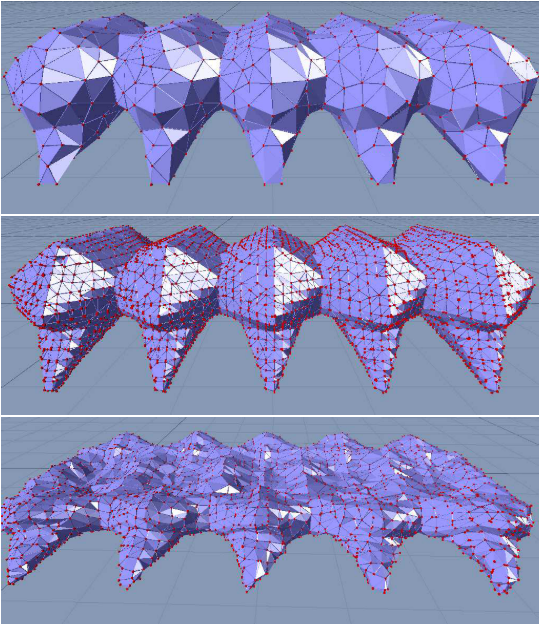
\includegraphics[width=1\linewidth]{Rieffel.png}<3->%
        \end{subfigure}
        \begin{subfigure}{.23\textwidth}
            %\centering
            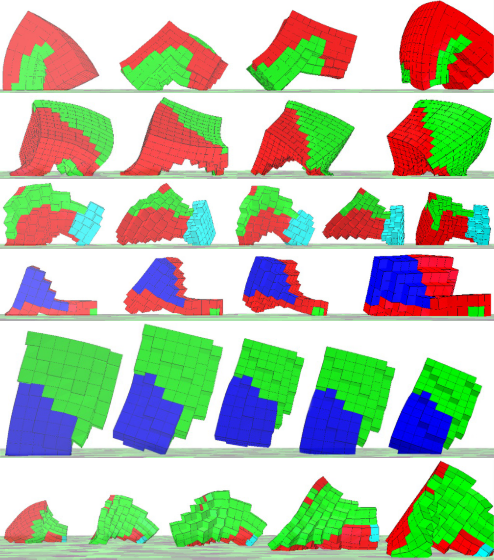
\includegraphics[width=1\linewidth]{Cheney.png}<4->%
        \end{subfigure}
        \begin{subfigure}{.5\textwidth}
            %\centering
            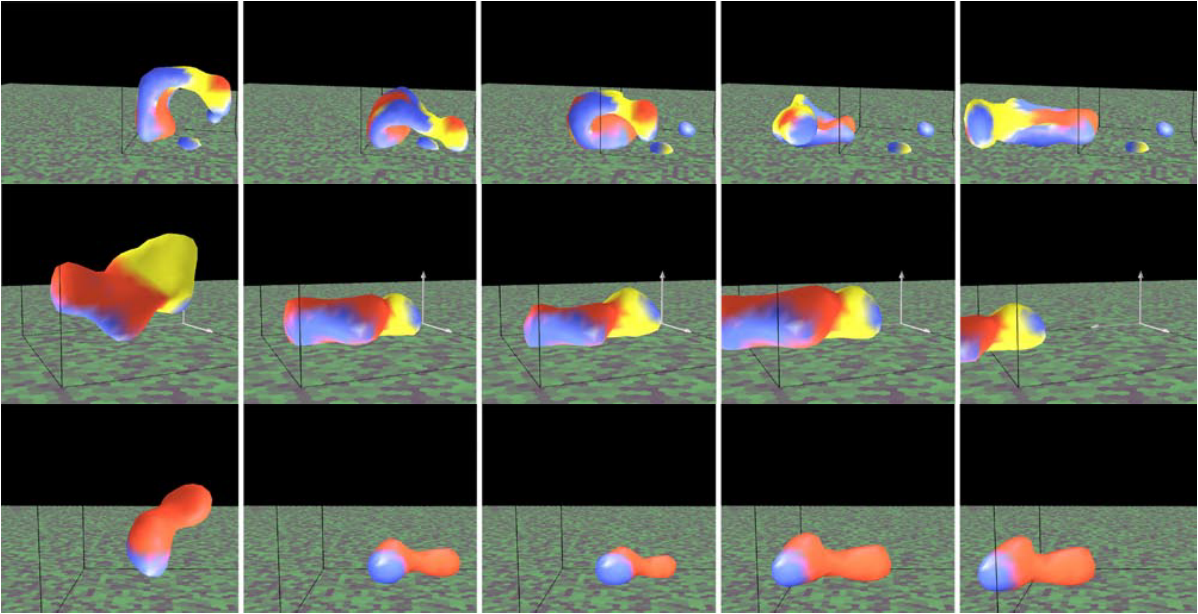
\includegraphics[width=1\linewidth]{Hiller.png}<5->%
        \end{subfigure}
    \end{figure}
\end{frame}

%   Background----------------------------------------------------%

\begin{frame}
    \frametitle{Background (cont.)}
    \begin{itemize}
        \item<1-> Lindenmayer systems (L-systems)
        \changefontsizes{11pt}
        \begin{itemize}
            \item<2-> Recursive grammatical encodings
            \item<3-> Built from axiom, variables, constants and rules
        \end{itemize}
    \end{itemize}
    \begin{figure}
        \centering
        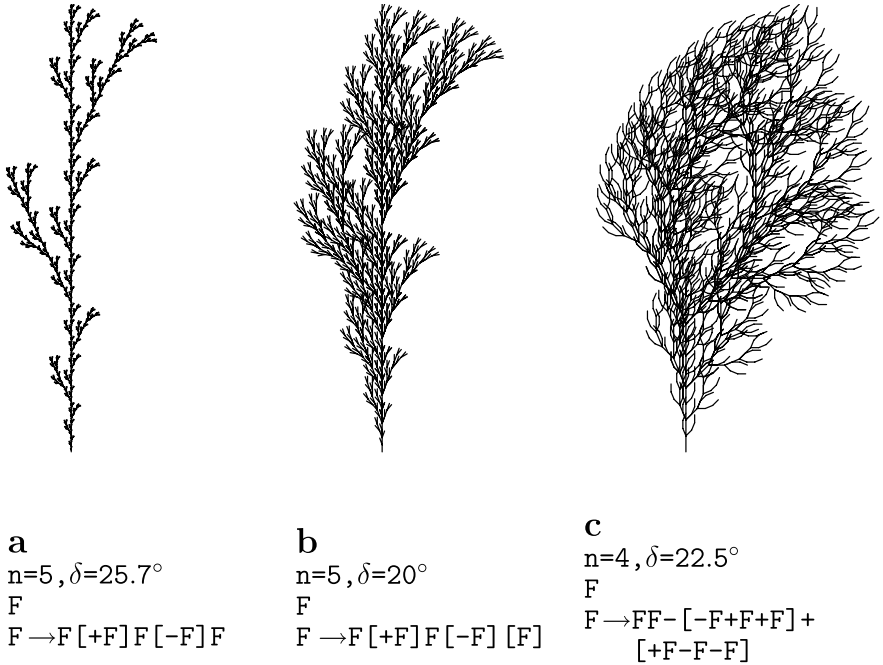
\includegraphics[height = 5cm]{L-Systems_Examples.png}<4->
    \end{figure}
\end{frame}

%   Background----------------------------------------------------%

\begin{frame}
    \frametitle{Background (cont.)}
    \begin{itemize}
        \item<1-> Compositional Pattern-Producing Network - NeuroEvolution of Augmenting Technologies (CPPN-NEAT)
        \changefontsizes{11pt}
        \begin{itemize}
            \item<2-> Neural networks
            \item<3-> Evolved with topology augmentation
        \end{itemize}
    \end{itemize}
    \begin{figure}
        \centering
        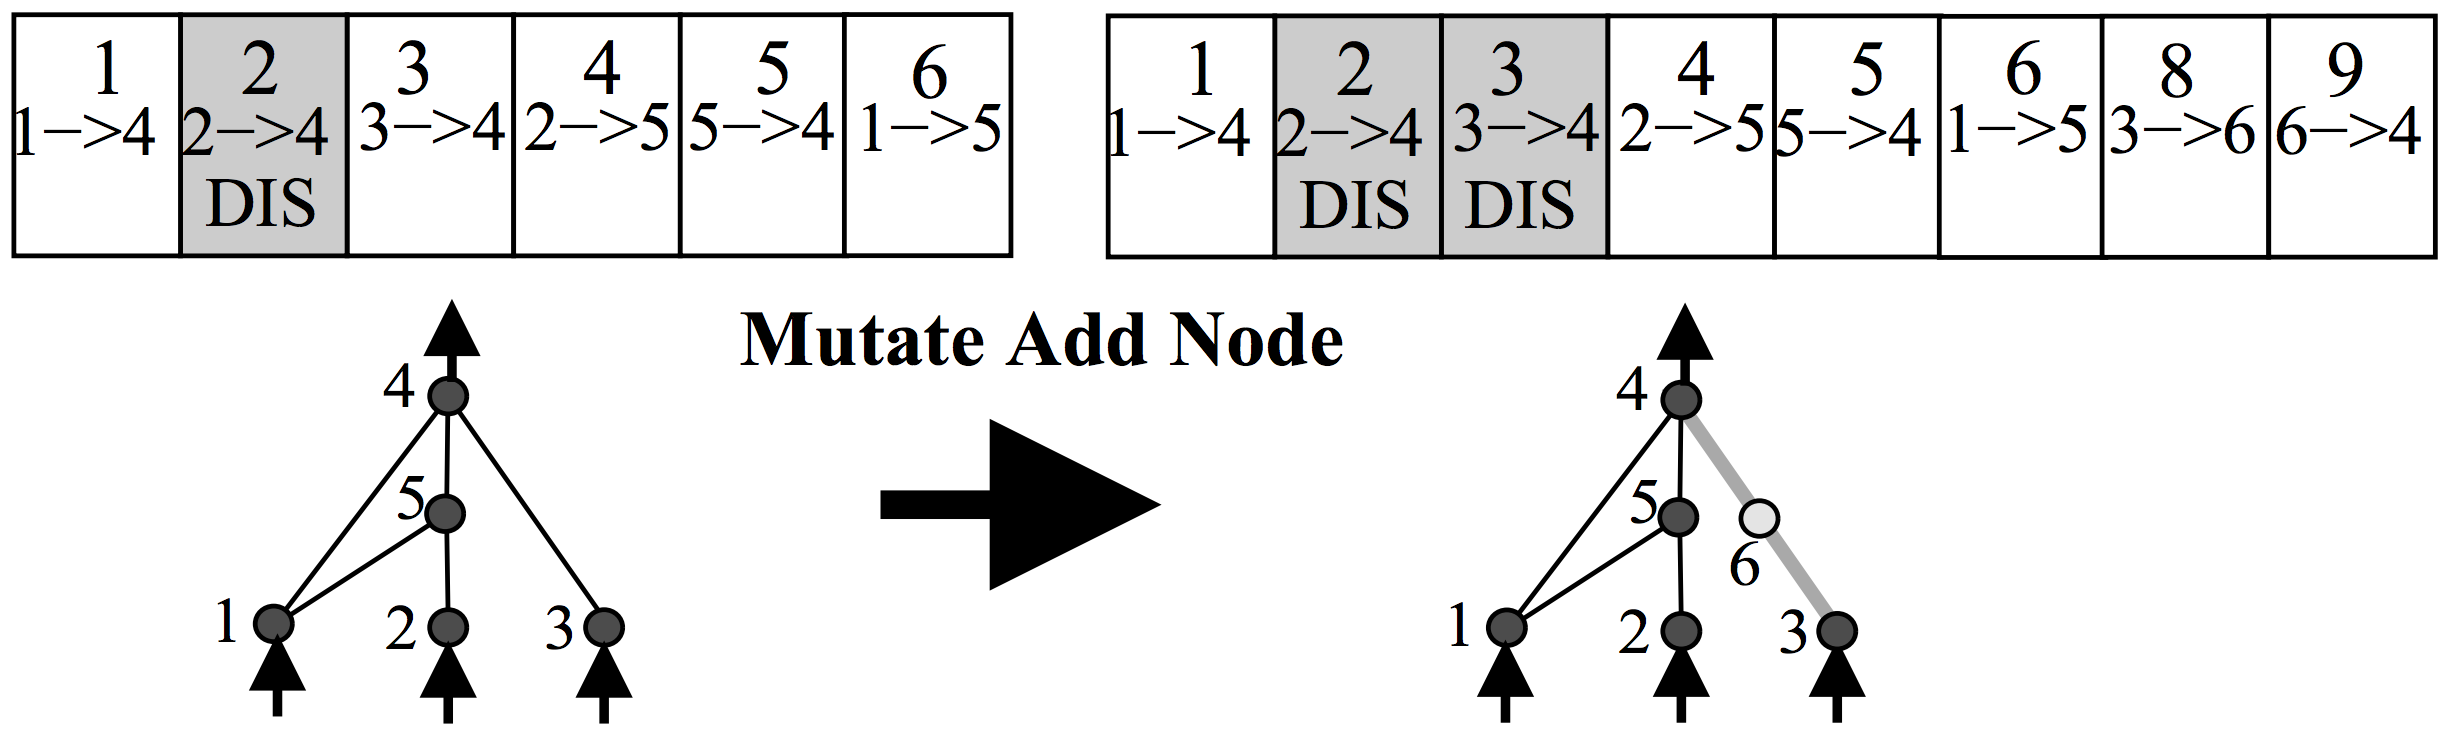
\includegraphics[height = 3cm]{CPPN_Topology_Augmentation.png}<4->
    \end{figure}
\end{frame}

%   Software------------------------------------------%

\begin{frame}
    \frametitle{Software}
    \begin{itemize}
        \item<1-> LSDyna
        \changefontsizes{11pt}
        \begin{itemize}
            \item<2-> Commercial software
            \item<2-> Support
            \item<3-> High level of control
            \item<3-> Robust
        \end{itemize}
    \end{itemize}
    \begin{figure}[ht!]
        \captionsetup{skip=0.333\baselineskip}
        \centering
        \begin{subfigure}{.49\textwidth}
            \centering
            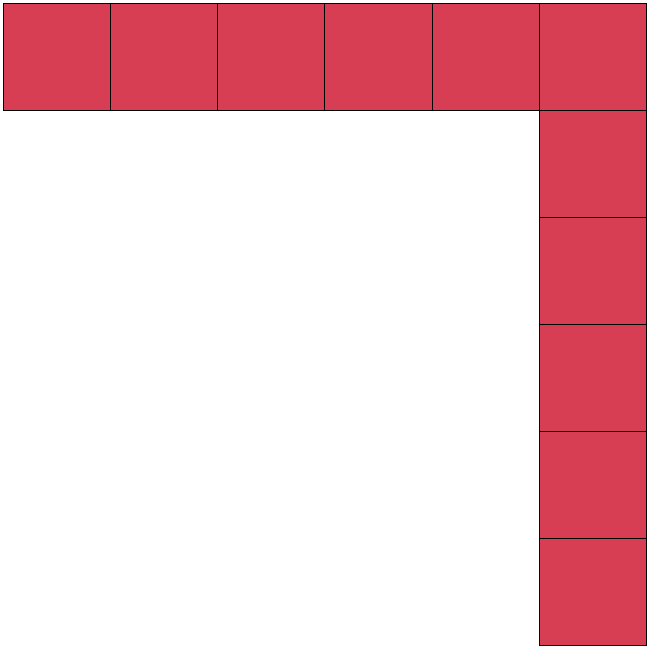
\includegraphics[width=0.5\linewidth]{Unit_Cell_Corner_Cropped.png}<4->
        \end{subfigure}
        \begin{subfigure}{.49\textwidth}
            \centering
            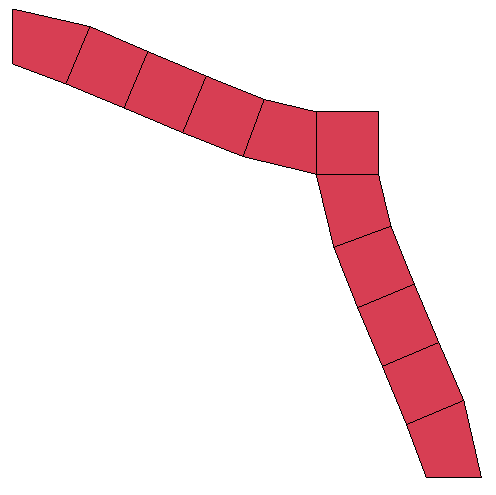
\includegraphics[width=0.6\linewidth]{Unit_Cell_Corner_Deformed.png}<4->
        \end{subfigure}
    \end{figure}
\end{frame}

%   Basic Structure------------------------------------------%

\begin{frame}
    \frametitle{Basic Structure}
    \begin{itemize}
        \item<1-> Unit cell
        \changefontsizes{11pt}
        \begin{itemize}
            \item<2-> Square
            \item<3-> Modelled with Mold Star 15
            \item<4-> Predefined behaviours
        \end{itemize}
    \end{itemize}
    \begin{figure}
        \centering
        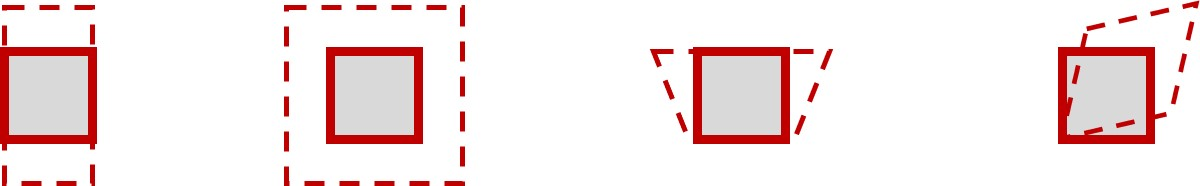
\includegraphics[height = 1.5cm]{Unit_Cell_Deformation.jpg}<4->
    \end{figure}
\end{frame}

%   Basic Structure------------------------------------------%

\begin{frame}
    \frametitle{Basic Structure (cont.)}
    \begin{itemize}
        \item<1-> Complete soft body
        \changefontsizes{11pt}
        \begin{itemize}
            \item<2-> Constructed from unit cells
            \item<5-> Recursive grammatical encodings
        \end{itemize}
    \end{itemize}
    \begin{figure}[ht!]
        \captionsetup{skip=0.333\baselineskip}
        \centering
        \begin{subfigure}{.49\textwidth}
            \centering
            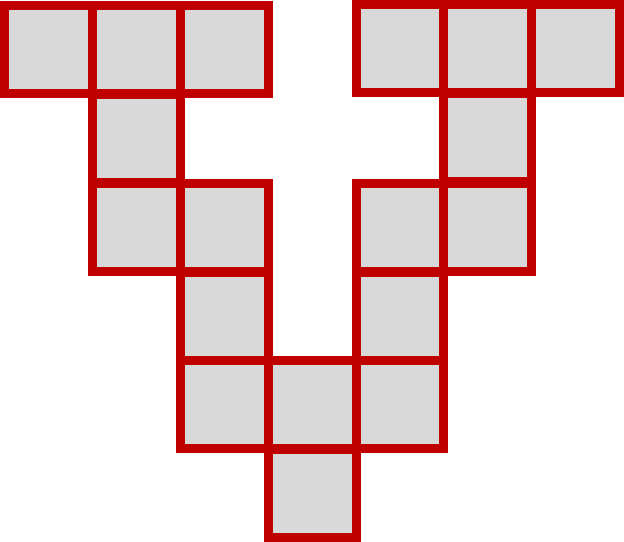
\includegraphics[width=0.6\linewidth]{Soft_Body_Undeformed.png}<3->
        \end{subfigure}
        \begin{subfigure}{.49\textwidth}
            \centering
            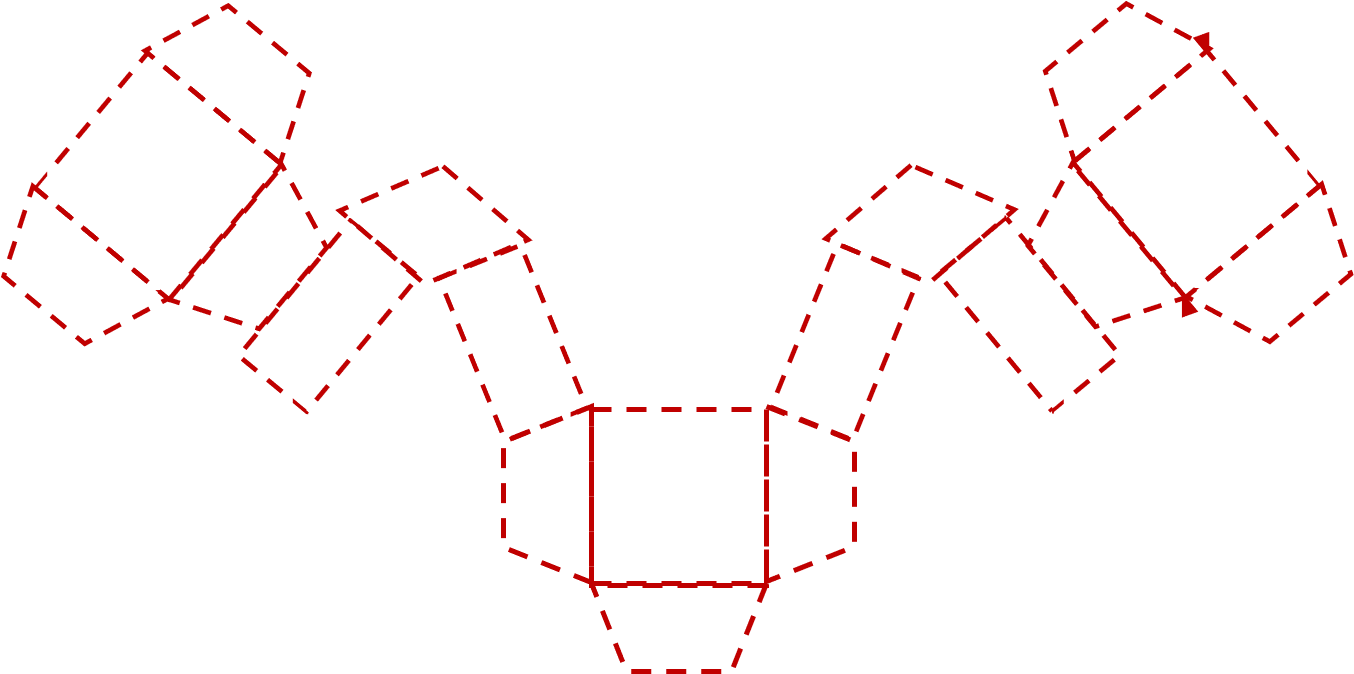
\includegraphics[width=1\linewidth]{Soft_Body_Deformed.png}<4->
        \end{subfigure}
    \end{figure}
\end{frame}

%   Recursive Encodings------------------------------------------%

\begin{frame}
    \frametitle{Recursive Encodings}
    \begin{minipage}{0.7\textwidth}
        \begin{itemize}
            \item<1-> L-systems
            \changefontsizes{11pt}
            \begin{itemize}
                \item<2-> Refer to unit cells
                \item<3-> Construct soft body
                \item<4-> Genotype
            \end{itemize}
            \item<5-> CPPN-NEAT
            \changefontsizes{11pt}
            \begin{itemize}
                \item<6-> Refer to whole body
                \item<7-> Phenotype
            \end{itemize}
        \end{itemize}
    \end{minipage}
    \begin{minipage}{0.25\textwidth}
    \begin{figure}
        \centering
        
\includegraphics[height = 3cm]{Genotype.png}<4->
    \end{figure}
    \begin{figure}
        \centering
        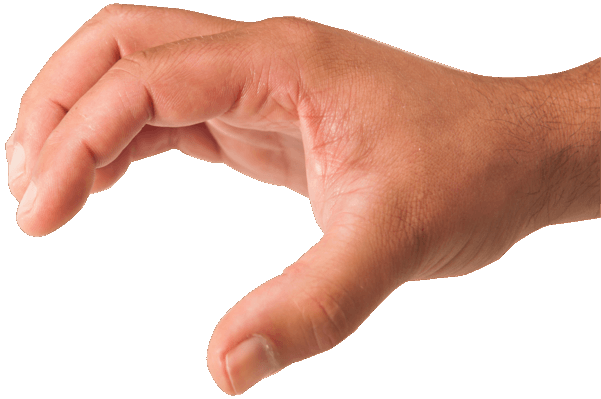
\includegraphics[height = 2cm]{Phenotype.png}<7->
    \end{figure}
    \end{minipage}
\end{frame}

%   Proof Of Concept------------------------------------------%

\begin{frame}
    \frametitle{Proof of Concept}
    \begin{itemize}
        \item<1-> Use material properties obtained from testing
        \item<2-> Manufacture physical model
        \changefontsizes{11pt}
        \begin{itemize}
            \item<3-> Unit cell and whole body
            \item<4-> Produce at some thickness
            \item<5-> Place between glass plates
            \item<6-> Apply internal pressure
            \item<7-> Observe behaviour
        \end{itemize}
    \end{itemize}
    \begin{figure}
        \centering
        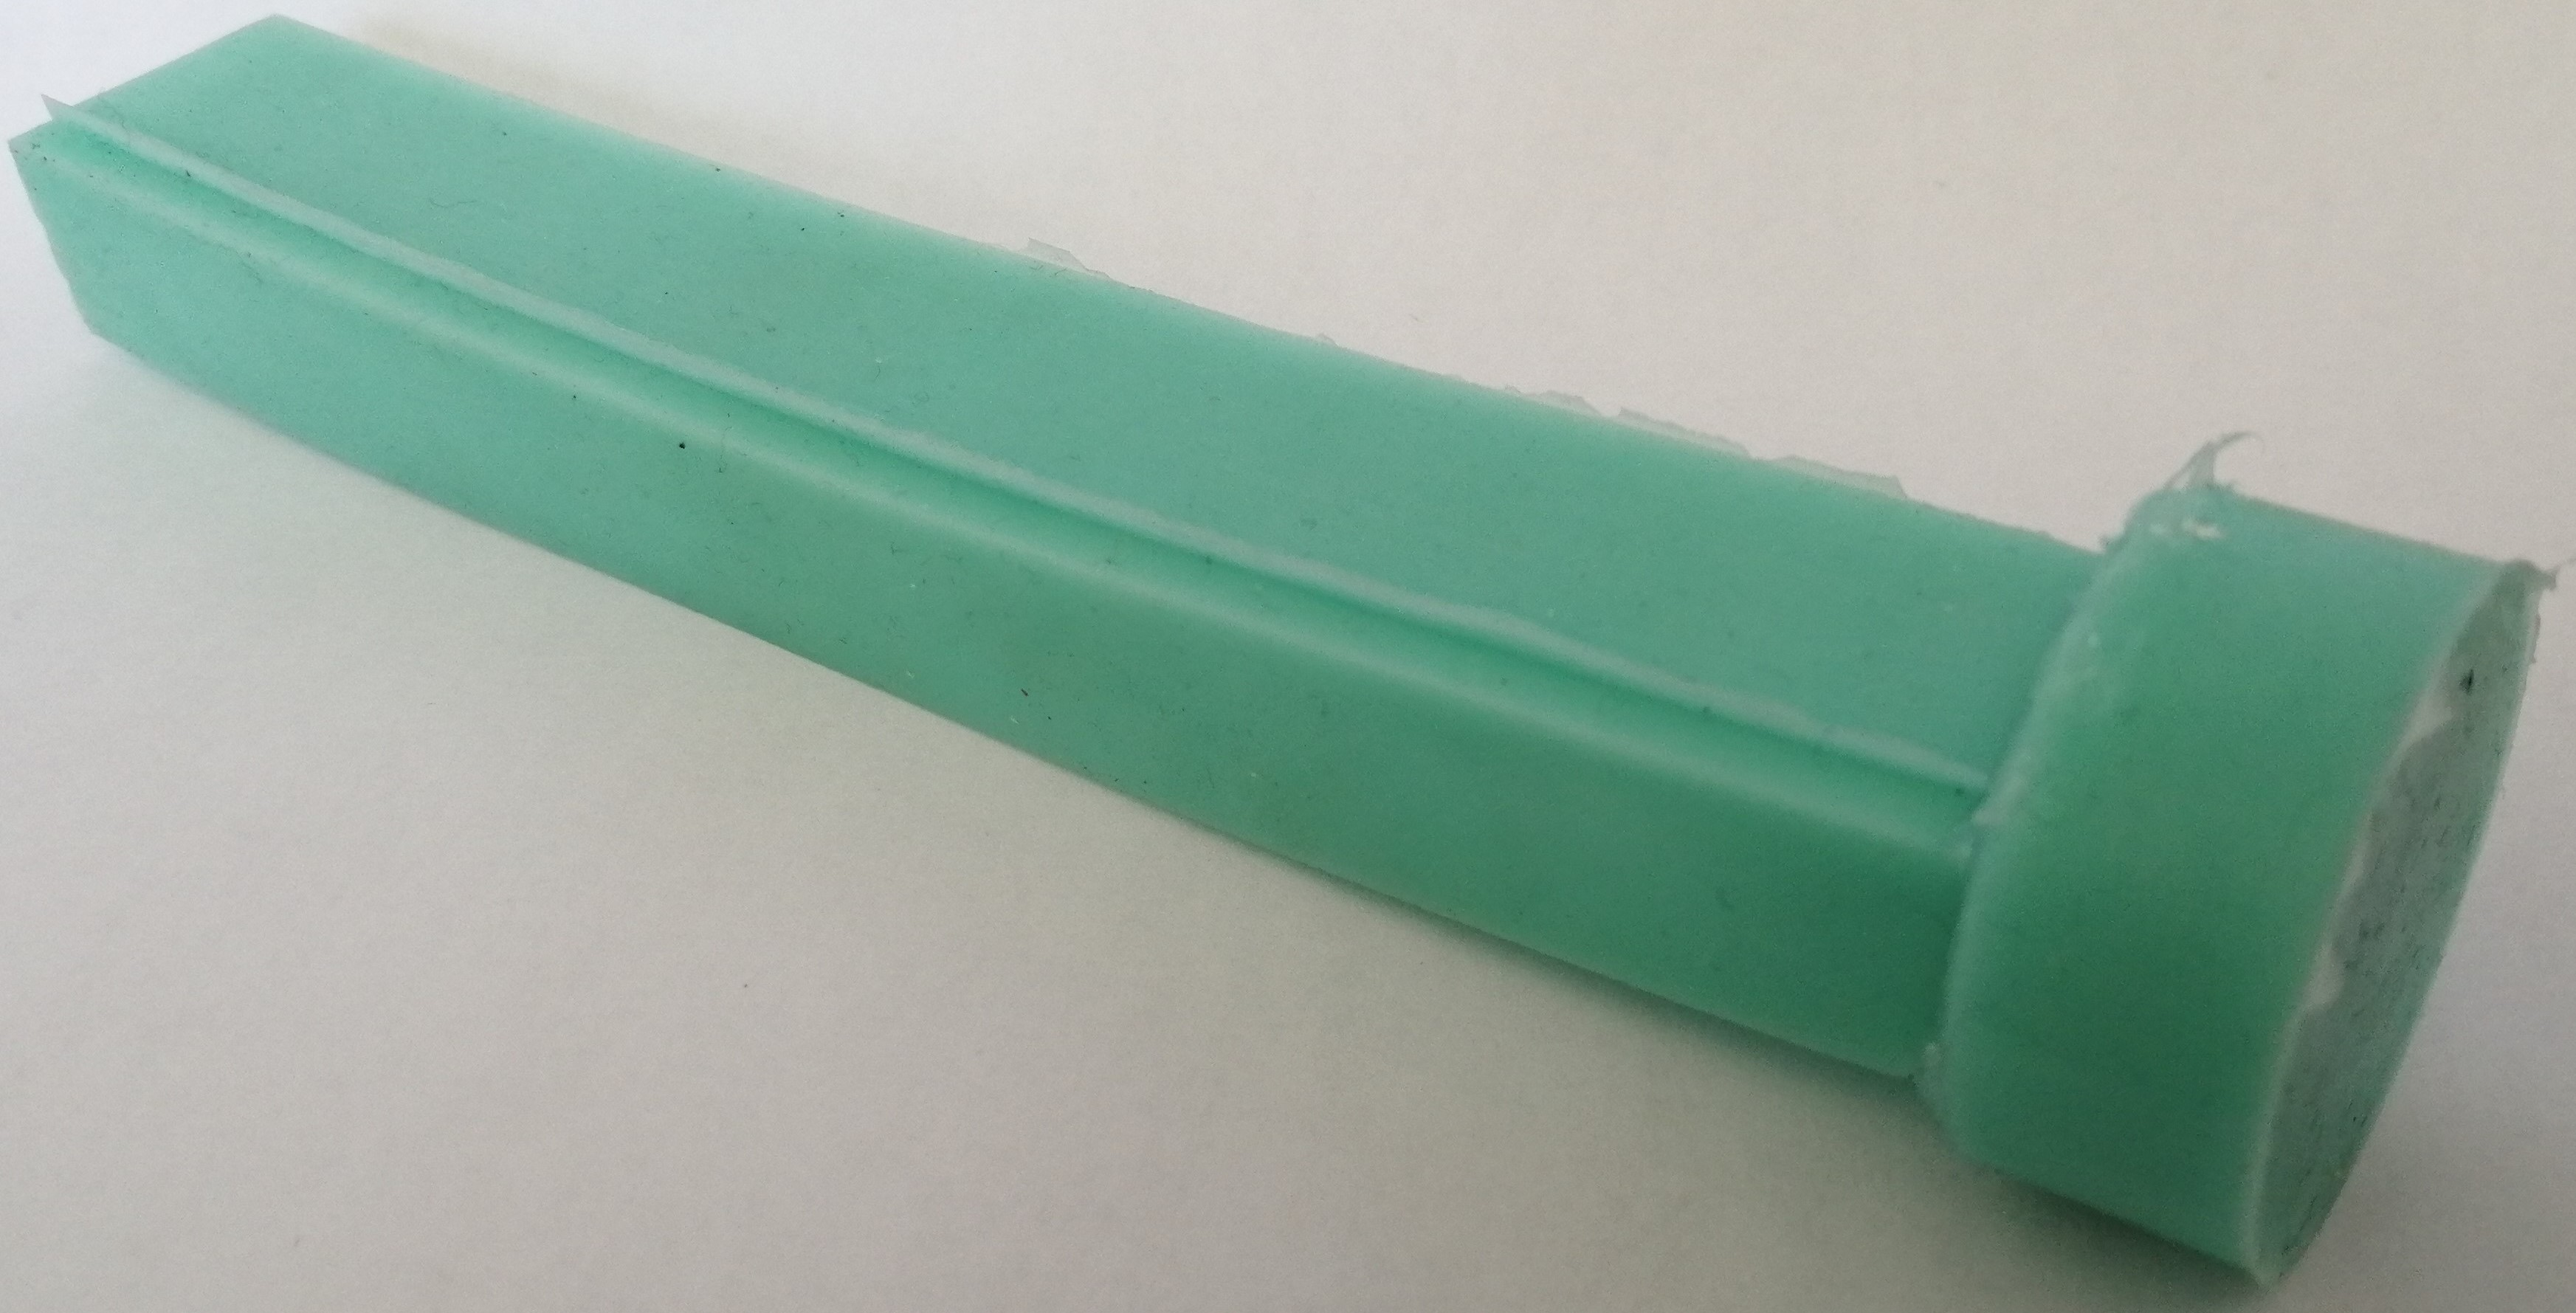
\includegraphics[height = 3cm]{Mold_Star_15.jpg}<1->
    \end{figure}
\end{frame}

%   Conclusions And Results------------------------------------------%

\begin{frame}
    \frametitle{Results and Conclusions}
    \begin{itemize}
        \item<1-> Improve computing time required
        \item<2-> Prove practicality of recursive encodings
        \item<3-> Replicable
        \item<4-> Adaptable
        \begin{itemize}
            \item<5-> 3D
            \item<6-> Different objective functions
        \end{itemize}
    \end{itemize}
\end{frame}

%   Questions---------------------------------------------------%

\begin{frame}
    \begin{center}
        \huge Questions?
    \end{center}
\end{frame}

\end{document}
